\documentclass[../diploma.tex]{subfiles}
 
\begin{document}

В сообществе специалистов в области машинного обучения последние годы прослеживается пока ещё незатухающий интерес к нейронным сетям. 
На многих публичных выступлениях любят говорит о том, что дешёвые GPU дали второе дыхание нейронным сетям. 
Вы часто услышите об открытых соревнованиях, на которых решения, основанные на глубинном обучении, добились такой точности, что отправили считавшуюся ранее открытой проблему в разряд решённых.
Одним из таких знаменитых примеров стало закрытие проекта Asirra\cite{elson2007asirra} в результате контекста на Kaggle\cite{kaggle:dogcats}. 

В этой работе мы не преследуем целей добиться выдающихся результатов с точки зрения точности модели.
Дело в том, что самые последние \hyperref[sec:existing_solutions]{исследования} \autoref{sec:existing_solutions} в сфере генерации голоса публикуются исследовательскими командами крупных корпорации с большими вычислительными ресурсами. 

Статья \cite{article:van2016wavenet}, на результатах которой основана данная работа не исключение.
Мы не собирались соревноваться в качестве генерации с существующими решениями. Мы, в свою очередь, постараемся развить идею придачи дополнительных характеристик генерируемому голосу. Такие характеристики можно придумать самые разные: от простого мужской/женский голос до имитации речи конкретного человека.

% Мы, в свою очередь попытаемся реализовать необычное применение к старым методам. 
% Причём наши исследования воспроизводимы даже в домашних усслових для более или менее пт риличной конфигурации ПК.

% Хотелось бы внести свой вклад в 
Инструментарий для таких целей предоставляет публикация WaveNet: A Generative Model for Raw Audio \cite{article:van2016wavenet}, однако только с точки зрения архитектуры и совсем без описания дополнительных признаков. Мы посчитали, что более подробное исследование этого вопроса и получение практических результатов было бы достойным вкладом в исследовательское сообщество.

\subsection*{Практическая ценность}

Модель, которую мы хотим построить в перспективе может найти множество практических применений от персонализированного голоса в навигаторе до эмуляции голосов знаменитостей. Конечно разработка такой полноценной промышленной системы самостоятельная сложная задача, выходящая далеко за рамки данной работы. Однако мы должны понимать, как должен выглядеть внешний интерфейс взаимодействия с моделью, чтобы последняя была полезна на практике. 

Высокоуровневый макет предполагаемой системы изображен на рисунке \ref{fig:speech_system}.

\begin{figure}[h!]
  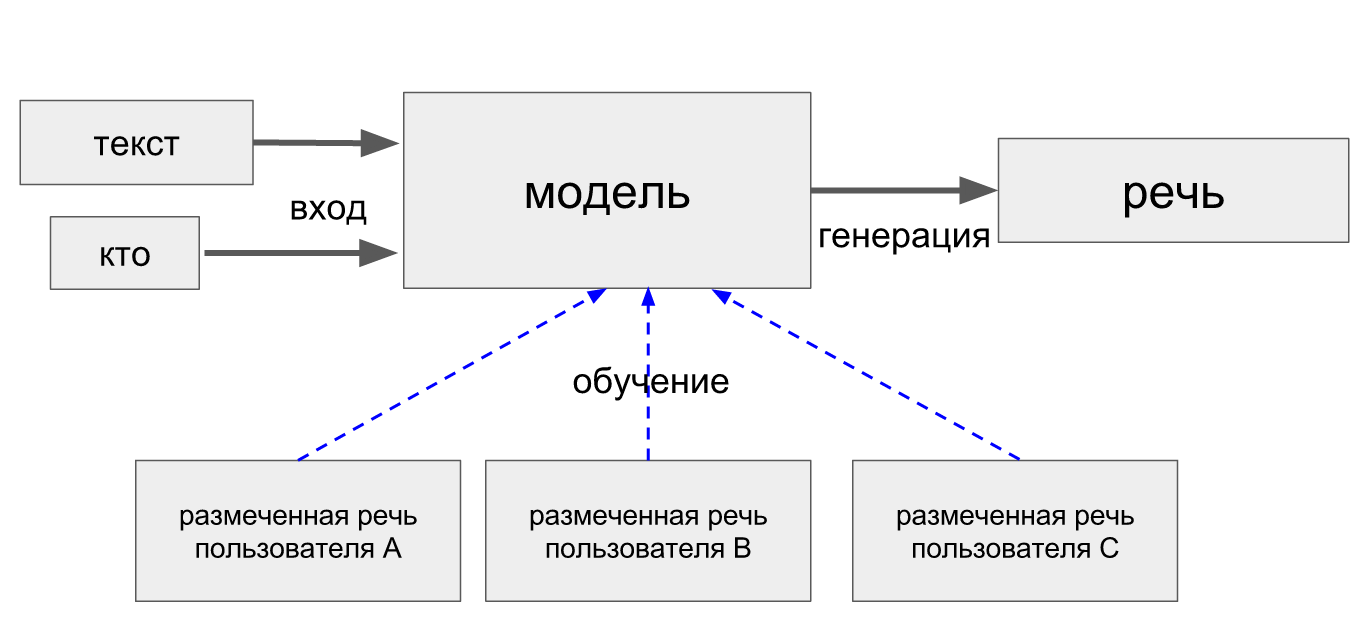
\includegraphics[scale=0.36]{img/scheme}
  \caption{Система генерации речи}
  \label{fig:speech_system}
\end{figure}

\pagebreak
\end{document}

Опишем, каким бы мы хотели видеть сценарий использование системы, в предположении что подлежащая модель работает идеально.
Изображенная система должна быть заранее обучена на некоторой базе пользователей, для каждого из которых  предоставлено достаточное количество записей голоса вместе с выровненным вдоль звука произносимым текстом. 

На вход должен подаваться текст, вместе с дополнительными признаками, которые мы назовём \textbf{локальные условия} и некоторой общей харакеристкой, к примеру, описывающей, чей голос мы хотим сгенерировать. Такую характеристику назовём \textbf{глобальным условием}. 

На выходе возвращается речь с ожидаемыми особенностями.